% Revised Section II.B based on the originally uploaded source.
% The grid-sensitivity table is included directly in this file so that
% replacing the B-section source also updates the medium-grid count.
% Verify the reported cell counts against the actual mesh files before submission.

\subsection{CFD Setup and Convergence Assessment}
\label{sec:cfd-setup}

\subsubsection{Numerical Method}
\label{sec:numerical-method}

The aerodynamic databases were generated using ADflow, an open-source structured multiblock finite-volume solver for compressible aerodynamic analysis \cite{Mader2020ADflow}. The steady Reynolds-averaged Navier--Stokes (RANS) equations were solved with the Spalart--Allmaras turbulence model. The wing surface was treated as an adiabatic no-slip wall, with symmetry conditions imposed on the half-wing symmetry plane and freestream conditions prescribed at the far-field boundaries. The convective terms were discretized using central differencing with scalar artificial dissipation. Each solution was initialized using Runge--Kutta iterations, followed by the approximate Newton--Krylov (ANK) algorithm described by Yildirim et al.~\cite{Yildirim2019ANK}. The solution was subsequently advanced to convergence using Newton--Krylov (NK) iterations. Twenty turbulence subiterations were performed during each nonlinear iteration. The convergence criterion was defined as a reduction of at least ten orders of magnitude in the normalized total residual, $R/R_0\leq10^{-10}$, where $R_0$ is the initial residual.

\subsubsection{Grid Configuration and Sensitivity Assessment}
\label{sec:grid-sensitivity}

The infinite-span swept-wing calculations employed a two-block structured
sectional mesh with 333 circumferential and 97 wall-normal points.
The \SI{10}{m} constant-chord finite-wing knowledge-domain cases used the
same $333\times97$ sectional resolution, with additional discretization
in the spanwise direction. The sectional mesh included 296 points along
the airfoil surface, with additional clustering near the leading and
trailing edges, and 19 points in the wake region. The near-wall spacing
was selected to maintain $y^{+}<1$. For the infinite-span configurations,
the far-field boundary was located approximately $30c$ from the airfoil,
and the wall-normal spacing increased gradually toward the far field.
Although the infinite-span and finite-wing knowledge-domain cases shared
the same sectional resolution, their full computational meshes differed
because the finite-wing calculations required spanwise discretization.

A three-level grid-refinement study was conducted before database
generation to evaluate the spatial-discretization sensitivity of the
finite-wing solutions. A representative constant-chord swept wing was
selected with a thickness-to-chord ratio of $t/c=0.1195$, a quarter-chord
sweep angle of $\Lambda_{c/4}=33.33^\circ$, a chord of $c=\SI{1}{m}$,
and a semispan of $b/2=\SI{10}{m}$. The corresponding flow condition was
$M_\infty=0.76$, $\alpha=2.0^\circ$, and $Re_c=6.1686\times10^6$.
The three-dimensional grids employed a five-block topology, a first-cell
height of $5\times10^{-6}c$, and a far-field boundary located at $50c$.
The surface mesh and the near-body symmetry-plane mesh of the medium grid
are shown in Fig.~\ref{fig:medium-grid}.

\begin{figure}[!htb]
    \centering
    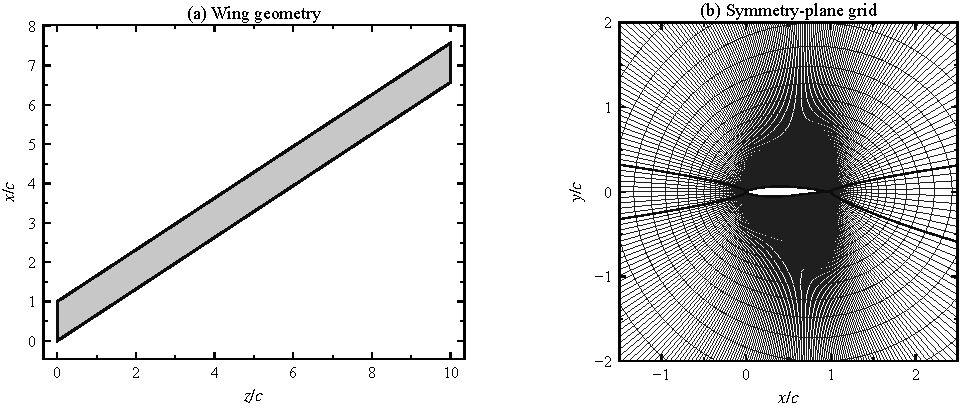
\includegraphics[width=0.94\linewidth]
        {II_Database_and_Preprocessing/figures/II_B_Fig04/II_B_Fig04_medium_grid.pdf}
    \caption{Medium grid used for the finite-wing calculations:
    (a) planform surface mesh and (b) near-body symmetry-plane volume mesh.}
    \label{fig:medium-grid}
\end{figure}

The coarse, medium, and fine grids retained the same block topology,
surface-node distribution strategy, near-wall spacing, and far-field
extent, while their resolutions were varied as summarized in
Table~\ref{tab:grid-sensitivity}. Here, $N_c$, $N_s$, and $N_n$ denote
the sectional (circumferential), spanwise, and wall-normal point counts,
respectively. The medium grid employed a $333\times97\times97$
resolution, including the same $333\times97$ sectional point counts as
the knowledge-domain meshes.

% The source manuscript reported 3.113 million cells for its medium grid.
% This number is retained pending confirmation from the corrected mesh log.
\begin{table}[!htb]
    \centering
    \caption{Grid sensitivity of the representative swept-wing case.}
    \label{tab:grid-sensitivity}
    \begingroup
    \setlength{\tabcolsep}{3pt}
    \footnotesize
    \resizebox{\linewidth}{!}{%
        \begin{tabular}{lcccccccc}
            \hline
            Grid & $N_c\times N_s\times N_n$ & Cells ($10^6$)
            & $C_L$ & $C_D$ & $C_{M_z}$
            & $|\Delta C_L|$ (\%) & $|\Delta C_D|$ (\%)
            & $|\Delta C_{M_z}|$ (\%) \\
            \hline
            Coarse & $261\times81\times81$ & 1.828
            & 0.390022 & 0.0116301 & 1.351364 & 0.263 & 0.213 & 0.269 \\
            Medium & $333\times97\times97$ & 3.113
            & 0.390872 & 0.0116498 & 1.354607 & 0.045 & 0.044 & 0.030 \\
            Fine & $375\times117\times117$ & 5.378
            & 0.391049 & 0.0116549 & 1.355009 & --- & --- & --- \\
            \hline
        \end{tabular}%
    }
    \endgroup
\end{table}

The integrated aerodynamic coefficients exhibited monotonic convergence
with grid refinement. Relative to the fine-grid solution, the medium-grid
differences were 0.045\% in $C_L$, 0.044\% in $C_D$, and 0.030\% in
$C_{M_z}$. The reported cell count increased by a factor of 1.73 from
the medium to the fine grid, while the changes in all three integrated
coefficients remained below 0.05\%. The medium grid was therefore
selected for database generation, reducing the reported cell count by
42.1\% relative to the fine grid while retaining nearly identical
integrated aerodynamic coefficients.

Because the surface pressure coefficient is a primary prediction target
of the present study, grid sensitivity was also assessed using local
pressure distributions. Figure~\ref{fig:cp-grid-sensitivity} compares
the $C_p$ distributions obtained on the three grids at representative
spanwise locations of $z=0.5$, $5.0$, and $9.5$~m.

\begin{figure}[!htb]
    \centering
    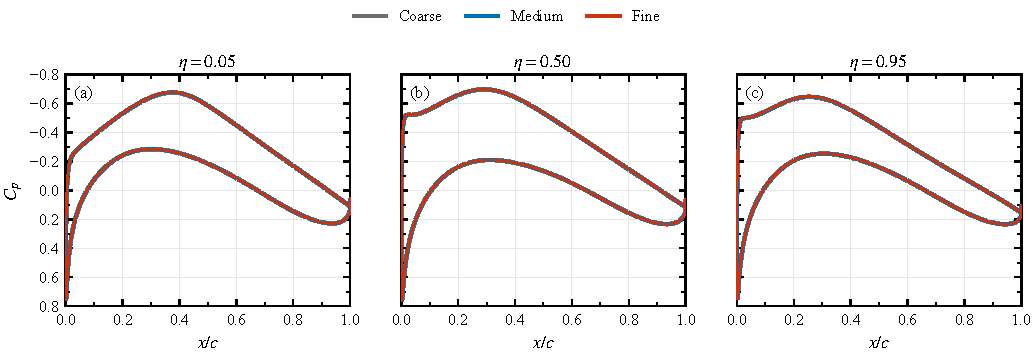
\includegraphics[width=0.94\linewidth]
        {II_Database_and_Preprocessing/figures/II_B_Fig05/II_B_Fig05_cp_grid_sensitivity.pdf}
    \caption{Pressure-coefficient distributions obtained on the coarse,
    medium, and fine grids at spanwise stations of $z=0.5$, $5.0$, and
    $9.5$~m for the representative finite-wing configuration.}
    \label{fig:cp-grid-sensitivity}
\end{figure}

The three locations exhibit distinct sectional loading characteristics,
whereas the medium- and fine-grid pressure distributions remain closely
matched. Together with the convergence of the integrated aerodynamic
coefficients, this agreement supports the use of the medium grid for the
finite-wing database calculations.

\subsubsection{Iterative Convergence Assessment}
\label{sec:solver-convergence}

In addition to the grid-sensitivity analysis, iterative convergence was
examined for the medium-grid verification case. Figure~\ref{fig:iterative-convergence}
shows the evolution of the normalized total residual, $R/R_0$, during
solution convergence.

\begin{figure}[!htb]
    \centering
    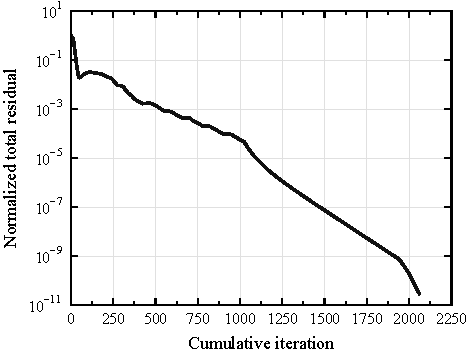
\includegraphics[width=0.72\linewidth]
        {II_Database_and_Preprocessing/figures/II_B_Fig06/II_B_Fig06_iterative_convergence.pdf}
    \caption{Convergence history of the normalized total residual for the
    medium-grid verification case.}
    \label{fig:iterative-convergence}
\end{figure}

The medium-grid solution converged after 2060 cumulative nonlinear
iterations. The normalized total residual decreased by 10.52 orders of
magnitude, satisfying the prescribed criterion of $R/R_0\leq10^{-10}$.
Over the final five reported iterations, the peak-to-peak variations in
$C_L$, $C_D$, and $C_{M_z}$ were 0.000059\%, 0.000013\%, and
0.000067\%, respectively. These variations were substantially smaller
than the corresponding medium-to-fine grid differences, indicating that
the remaining iterative error was negligible relative to the assessed
spatial-discretization sensitivity.
